\documentclass[11pt]{article}

\marginparwidth 0.5in 
\oddsidemargin 0.25in 
\evensidemargin 0.25in 
\marginparsep 0.25in
\topmargin 0.25in 
\textwidth=6in
\textheight=8in

\usepackage{listings}
\usepackage{xcolor}
\usepackage{graphicx}
\usepackage{caption}
\usepackage{subcaption}

\definecolor{codegreen}{rgb}{0,0.6,0}
\definecolor{codegray}{rgb}{0.5,0.5,0.5}
\definecolor{codepurple}{rgb}{0.58,0,0.82}
\definecolor{backcolor}{rgb}{0.95,0.95,0.95}

\lstset{
  backgroundcolor=\color{backcolor},
  commentstyle=\color{codegreen},
  keywordstyle=\color{magenta},
  numberstyle=\tiny\color{codegray},
  stringstyle=\color{codepurple},
  basicstyle=\ttfamily\footnotesize,
  breaklines=true,
  captionpos=b,
  numbers=left,
  numbersep=5pt,
  showstringspaces=false,
  tabsize=2,
  language=Python
}


\begin{document}
\hfill\vbox{\hbox{Jude Shin}
		\hbox{CSC 4888-S01-2268}	
		\hbox{Homework 3}	
		\hbox{\today}}\par

\bigskip
\centerline{\Large\bf Book Search}\par
\bigskip

\section{Explanation}

\subsection{Fitting the \lstinline{KNN} Model}

The code pre-processes the images and queries into gray-scale, essentially creating a useable vector (or embedding).
Then features were extracted from the image.
The features are in a high dimensional vector, and those are clustered using \lstinline{KMeans}.
We will be searching on the \lstinline{KMeans} centroids, not every document.
This makes searching our database more efficient.

Each of these clusters (or centroids) are converted into documents (aka, ``words").
Finally, these ``words" are converted into a histogram.
This is the final form that we will be comparing.
We save all of these histograms to the K-Nearest-Neighbors model using the \lstinline{.fit()} function.
Our ``search database" is finally ready to be used with real world images.

\subsection{Using the \lstinline{KNN} Model}

We use the same pre-process pipeline to get a histogram (or ``word").
Once we get an embedding that we can compare against, we get the closest 5 ``words" that are matches in our fitted \lstinline{KNN}.
The key is that we have to use the same \lstinline{KMeans} clustering model to get the same words that our \lstinline{KNN} is fitted on.
For each of the results that we got from the \lstinline{KNN} query, we just plot them out in a for loop in the end.

\section{Issues}

I got a bunch of weird results because I put everything to create a ``word" in a separate function (including the \lstinline{KMeans} model).
In turn, I used a completely new \lstinline{KMeans} object, resulting in completely different (and irrelevant) words.
I just got rid of the function entirely and just had some duplicated code.

I also ended up running out of compute time on Google Colab, so I wrote everything in one python script and ran it on my laptop.
It took forever, and when I messed something up, I would have to redo everything.
This was tedious and time consuming, but thankfully I didn't have to do that too many times.
This is why I added \lstinline{tqdm} to track the progress of each step.

\section{Discussion Questions}

\begin{enumerate}

	\item \textit{Evaluate how accurately the system is able to find the books in the query images.}

		It was pretty surprised with the accuracy of our model.
		For the first query, there were a lot of dogs in the photo that were similar, but not exactly a match with the query book.
		I also noticed that the feature detector that we created was pretty good at recognizing fonts.
		Titles are the most prominent on books; titles also have to get good contrast because they need to be readable, so I guess that is why there was good features that were extracted from them.
		Figures \ref{fig:query1}, \ref{fig:query2}, \ref{fig:query3}, \ref{fig:query4}, \ref{fig:query5}, \ref{fig:query6} show all 6 queries respectively.

	\item \textit{What do you notice about the search results that are not the same book as the query image? Are these search results related to the search query in some way?}
	
		Not in the same way (like text on the title of the book or such), but as I said before, the general theme could be seen in the images.
		Patterns like stars or animals or shapes are preserved through the covers.
		I thought that the results from the book "Are You My Mother" was pretty funny.
		The results had a lot of books with dogs on the picture, but only one out of the five were a correct match.
		I thought that was interesting.

	\item \textit{The two images in extra-queries are of books not included in the database. Test what happens when you search for these books.}

		The program doesn't just crash or something; it is pretty good at generalizing features.
		The themes that were talked about in the previous question are translated to these "unseen" images.
		The ``Piano" book seen in Figure \ref{fig:extra_query_1} got a similar piano teaching book on rank 5, which was cool.
		It wasn't the exact same book, but it had a similar graphic of a piano with wings.

		The other query seen in Figure \ref{fig:extra_query_2} image had a lot of sharp bold text that took up a good chunk of the cover.
		The 5 matches that were returned had all of the same features mentioned before, however, none were the same book.

	\item \textit{Can you think of a way to automatically determine if the search was successful, or if the book being searched is not in the database?}

		We could look at the distance and add some threshold.
		If the \lstinline{KNN} algorithm gives the closest match as being extremely large, then we can assume that query was not a known book.
		
\end{enumerate}

\section{Sources Used}

I used the \lstinline{skimage} documentation for the \lstinline{KMeans} and the \lstinline{TfidfVectorizer} packages.
I had some issues with when to use \lstinline{TfidfVectorizer.fit_transform} and \lstinline{TfidfVectorizer.transform}, so I had to do some digging on Google.

I also had some issues with running this code in Google Colab; I ran out of compute time with the number of images that we were processing.

\begin{figure}
	\centering
	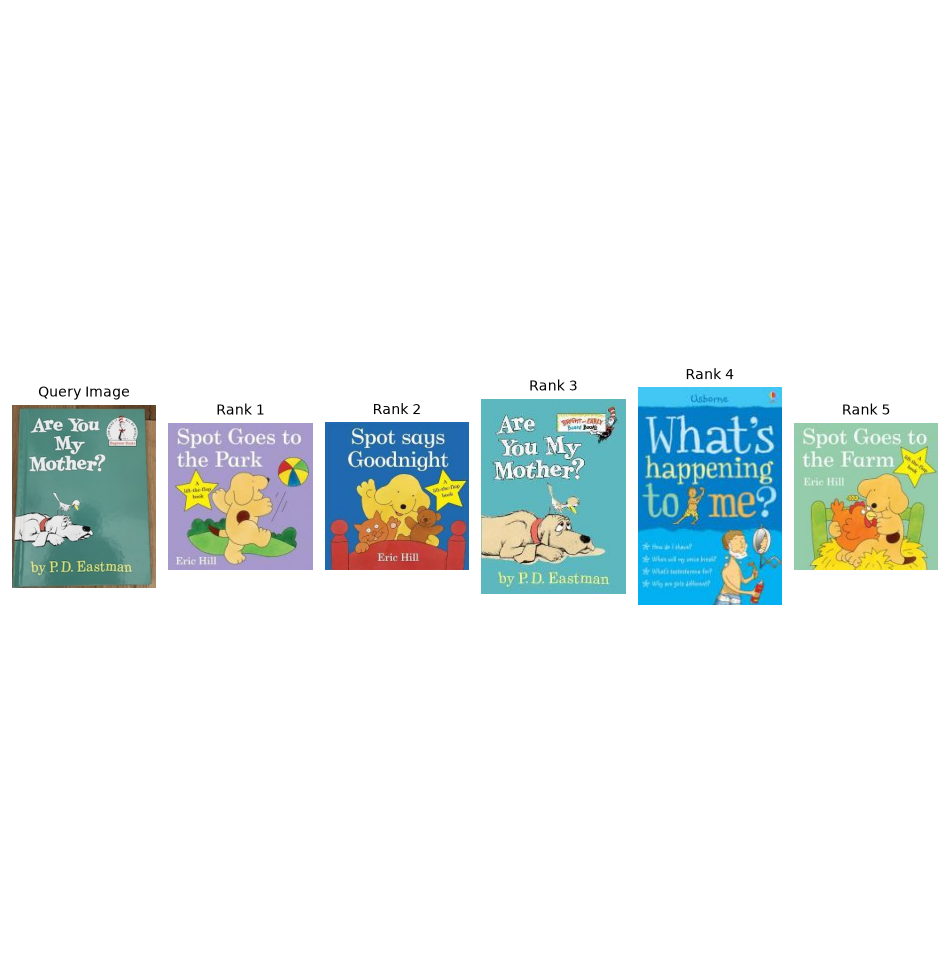
\includegraphics[width=0.8\textwidth]{assets/Figure_1.png}
	\caption{The third ranked result was a correct match.}
	\label{fig:query1}
\end{figure}

\begin{figure}
	\centering
	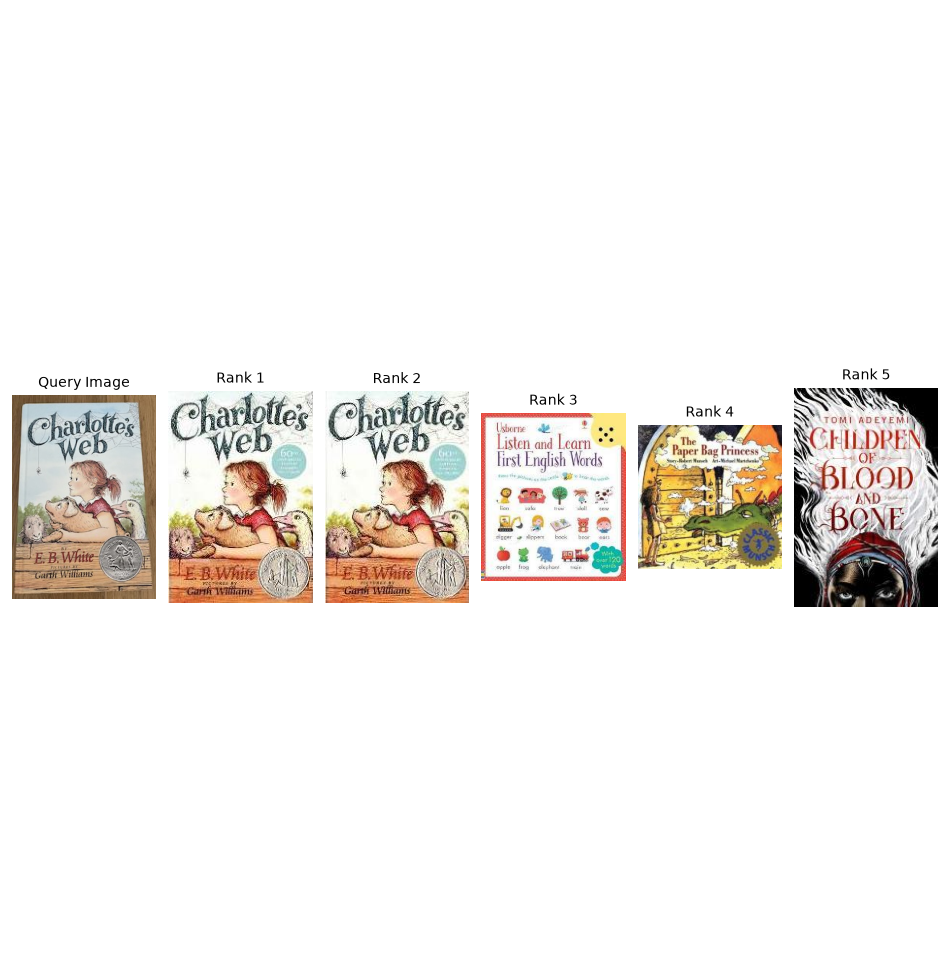
\includegraphics[width=0.8\textwidth]{assets/Figure_2.png}
	\caption{The first two ranked results were correct matches.}
	\label{fig:query2}
\end{figure}

\begin{figure}
	\centering
	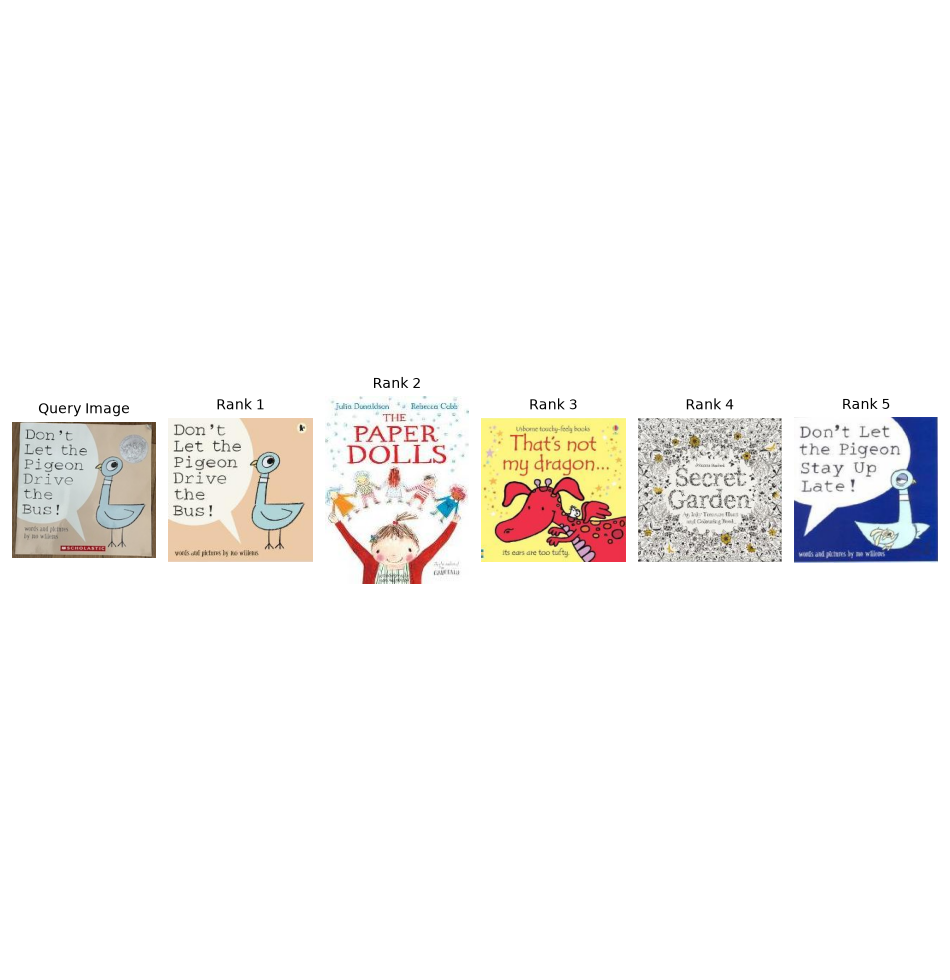
\includegraphics[width=0.8\textwidth]{assets/Figure_3.png}
	\caption{The first ranked result was a correct match.}
	\label{fig:query3}
\end{figure}

\begin{figure}
	\centering
	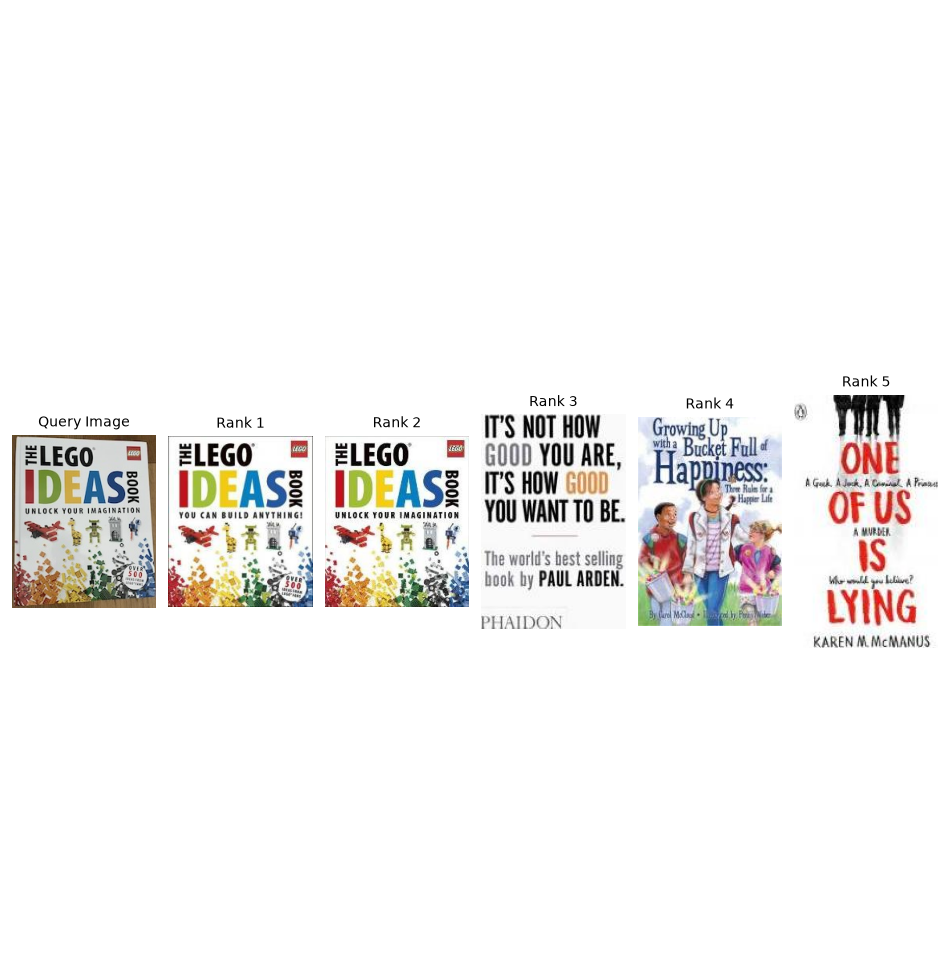
\includegraphics[width=0.8\textwidth]{assets/Figure_4.png}
	\caption{The first two ranked results were correct matches.}
	\label{fig:query4}
\end{figure}

\begin{figure}
	\centering
	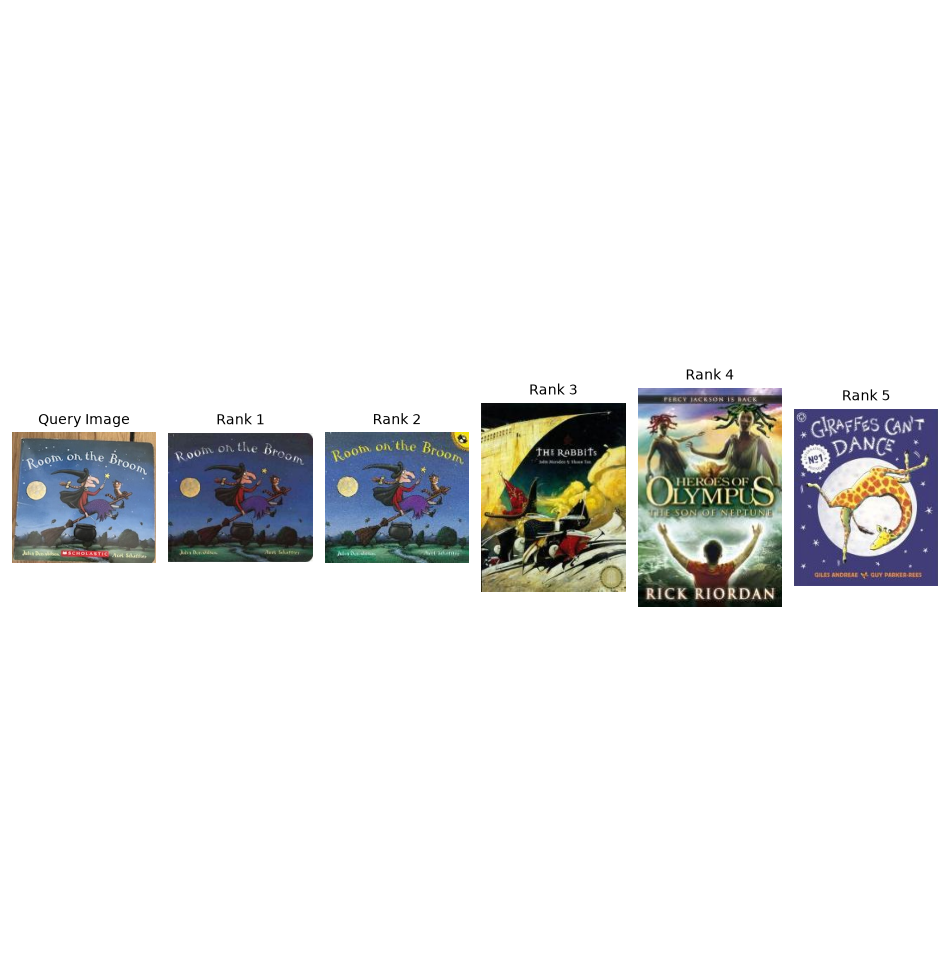
\includegraphics[width=0.8\textwidth]{assets/Figure_5.png}
	\caption{The first two ranked results were correct matches.}
	\label{fig:query5}
\end{figure}

\begin{figure}
	\centering
	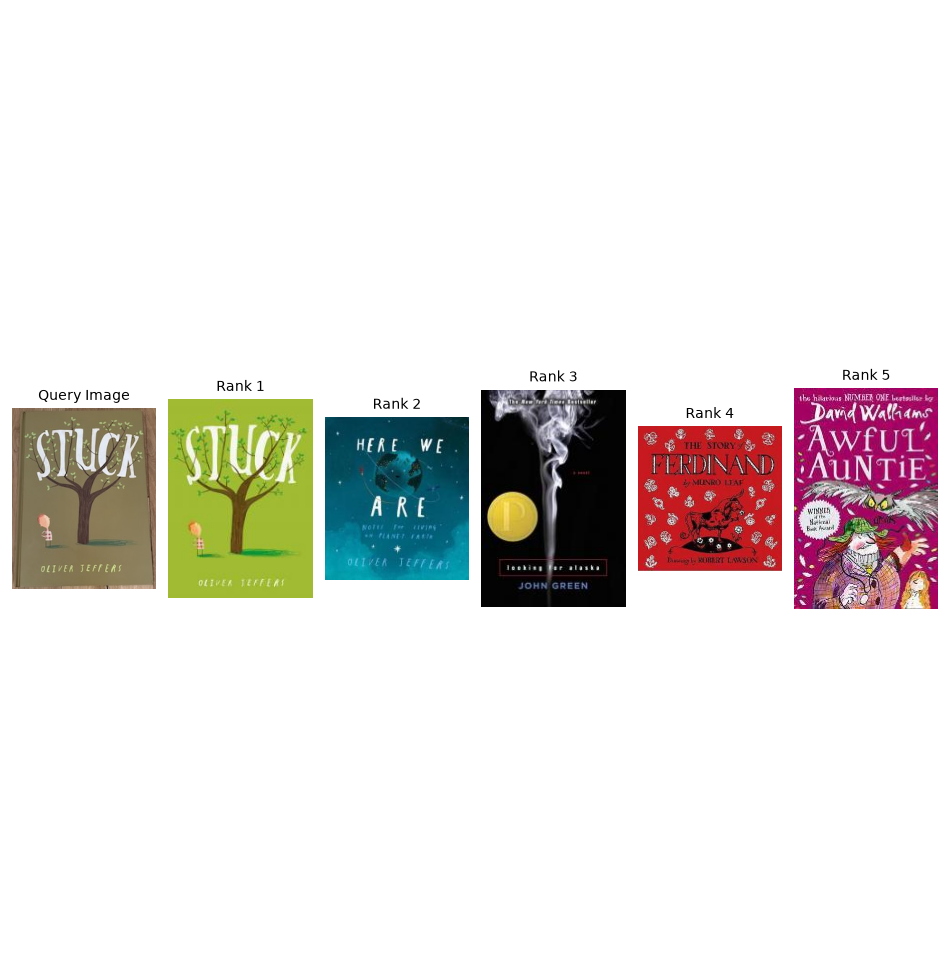
\includegraphics[width=0.8\textwidth]{assets/Figure_6.png}
	\caption{The first ranked result was a correct match.}
	\label{fig:query6}
\end{figure}

\begin{figure}
	\centering
	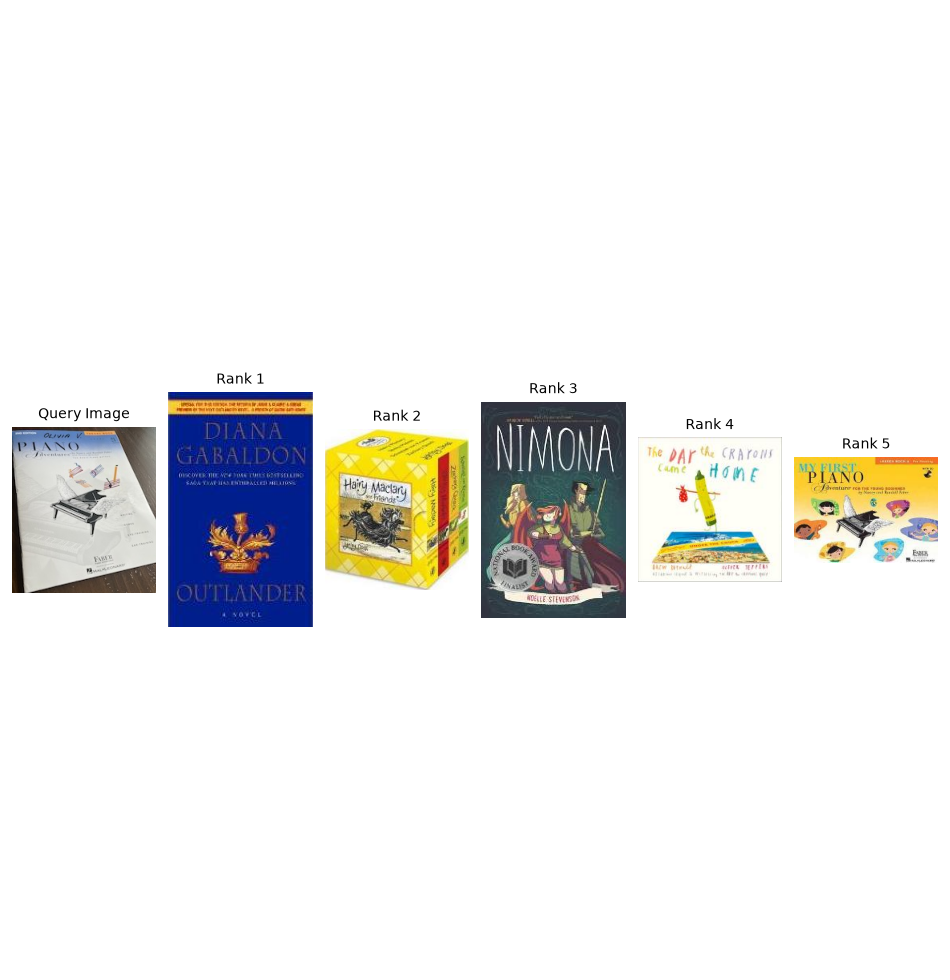
\includegraphics[width=0.8\textwidth]{assets/Figure_2_unseen.png}
	\caption{The same piano with wings can be seen in result with rank 5.}
	\label{fig:extra_query_1}
\end{figure}

\begin{figure}
	\centering
	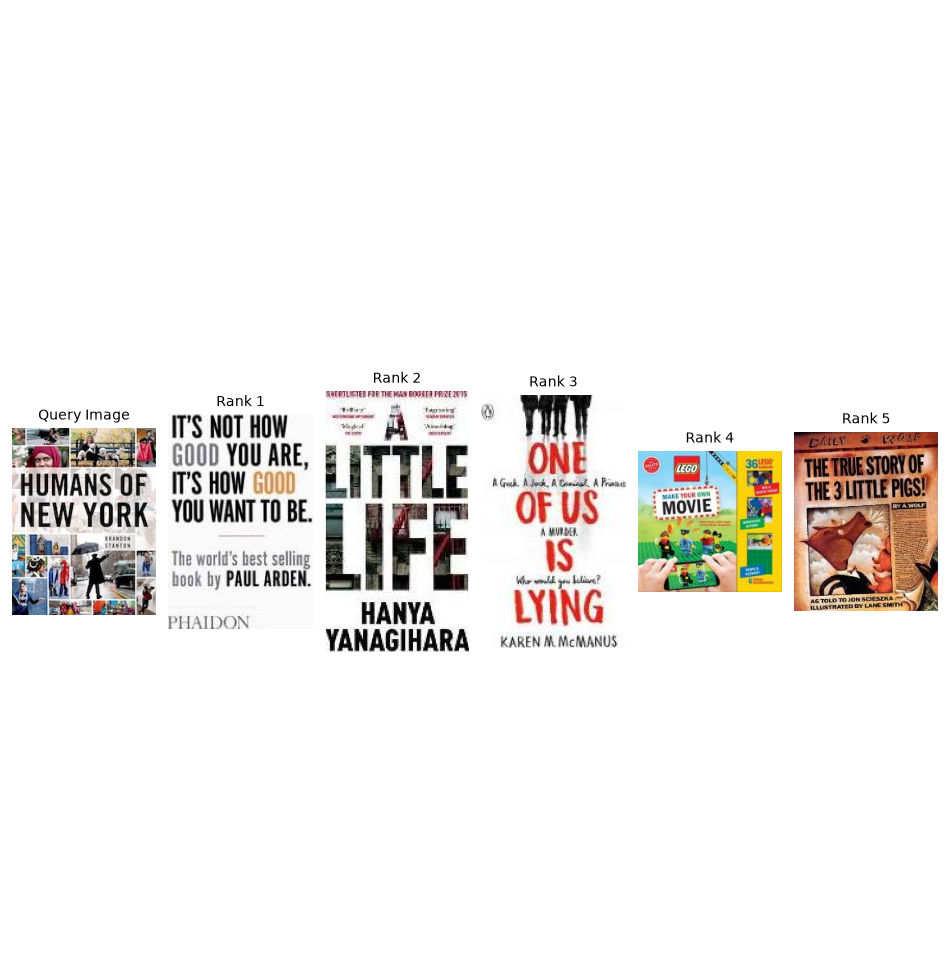
\includegraphics[width=0.8\textwidth]{assets/Figure_1_unseen.png}
	\caption{A common pattern of large bold text can be seen across most of the results.}
	\label{fig:extra_query_2}
\end{figure}

\end{document}
